\documentclass{article}
\usepackage[utf8]{inputenc}

%\title{Propuesta de Tesis: Individualizaci\'on de filamentos en una red mediante grafos.}
\title{Propuesta de Tesis: Individualizaci\'on de filamentos en una red mediante optimizaci\'on}
%\author{Leonardo Pizarro}
\date{}

\usepackage{natbib}
\usepackage{graphicx}
\usepackage{subcaption}
\renewcommand\refname{Referencias}
\begin{document}

\maketitle

\section{Contexto}
\label{contexto}
% aclarar rol de la entrada al método. Importancia de la imagen respecto al grafo
% En la propuesta se plantea desarrollar un método para extracción de filamentos, pero no queda claro cuál es la entrada al método, es un grafo o un imagen. Si es un grafo, la imagen juega algún papel importante?

En la naturaleza, es posible encontrar de forma ubicua, estructuras alargadas (filamentos), las que conforman redes entre sí. La conformación de estas estructuras complejas y din\'amicas se puede observar en ejemplos particulares como en una red de prote\'inas de una c\'elula eucariota, as\'i como en bacterias, ya que a pesar que pertenecer a distintas familias, ambas tienen estructuras formada por filamentos. 
Caracter\'isticas f\'isicas de estas redes generan propiedades tales como la presencia o ausencia de ciclos, o la posibilidad de dividir o no cada filamento. Por su parte, el análisis de filamentos que conforman la red, puede indicar el estado de \'esta, respecto a su ambiente o de su interior, as\'i como develar informaci\'on relevante sobre la relaci\'on entre la estructura biol\'ogica y funciones fisiol\'ogicas.  
%movimiento interno, reparación de tejido,
% estructuras dinamicas y complejas que juegan varios roles
% A modo de ejemplo, una red de proteinas de una c\'elula eucariota contiene tres tipos de filamentos en la constituci\'on de su citoesqueleto: microfilamentos, microt\'ubulos y filamentos intermedios. Sin embargo, una estructura de citoesqueleto también existe en una bacteria.
  
\vspace{.5cm}
Los m\'etodos actuales para analizar las redes mencionadas se basan en el procesamiento directo de im\'agenes obtenidas a partir de microscop\'ia (Figura \ref{Fig1a}), pasando por etapas de segmentaci\'on (Figura \ref{Fig1b}), para luego utilizar diversas t\'ecnicas como esqueletonizaci\'on (Figura \ref{Fig1c}), la transformada de Rad\'on o {\it template matching}. Esto permite identificar el grafo que representa a la red (Figura \ref{Fig1d}) o sirve de base para el uso de heur\'isticas que permiten identificar los filamentos de forma individual.
 %como tambi\'en pueden utilizarse una esqueletonizaci\'on de la misma (Figura \ref{Fig1c}), o la construcci\'on de un grafo (Figura \ref{Fig1d}), entre otras.
 % En todos estos casos, el objetivo radica en
La individualizaci\'on de filamentos permite cuantificar las propiedades de la red tales como n\'umero de filamentos, largo de estos, volumen, o curvatura. Estos m\'etodos, basados en la observaci\'on mediante microscop\'ia \'optica tienen como cota m\'axima de resoluci\'on el l\'imite de difracci\'on, $\lambda/2$. Donde $\lambda$ es la longitud de onda de la luz utilizada (o color). Este l\'imite establece que 2 objetos cuya distancia sea inferior a $\lambda/2$ no pueden ser diferenciados, conllevando a que dos partes del grafo cercanos puedan ser observadas como una, dificultando su estudio. Lo anterior es relevante para asociar las propiedades de la red a los v\'ertices del grafo extra\'ido, dando pie a la caracterizaci\'on del mismo (Figura \ref{Fig2a}).
 % vertices del grafo extraido, que representan a un filamento de forma individual, 
 
 \begin{figure*}[h!]
    \centering
    \label{fig:flujo-expected}
    \begin{subfigure}[t]{0.5\textwidth}
        \centering
        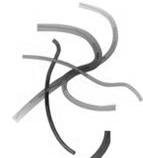
\includegraphics[height=1.5in]{define-weighted-4.png}
        \caption{Representaci\'on simplificada de una red con cruces y sobreposici\'on de filamentos en una imagen de microscop\'ia.}
        \label{Fig1a}
    \end{subfigure}%
    ~ 
    \begin{subfigure}[t]{0.5\textwidth}
        \centering
        
\includegraphics[height=1.5in]{define-weighted-4-bw-invert.png}
        \caption{Preprocesamiento de la imagen mediante segmentaci\'on para la extracci\'on de la red.}
        \label{Fig1b}
    \end{subfigure}
    %\caption{Caption place holder}
%\end{figure*}
\vskip\baselineskip
%\begin{figure*}[t!]
%    \centering
    \begin{subfigure}[t]{0.5\textwidth}
        \centering
        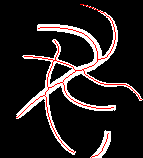
\includegraphics[height=1.5in]{skel_in_segment.png}
	    \caption{Esqueletonizaci\'on representativa de la red sobre la imagen de \ref{Fig1b}.}
        \label{Fig1c}
    \end{subfigure}%
    ~ 
    \begin{subfigure}[t]{0.5\textwidth}
        \centering
        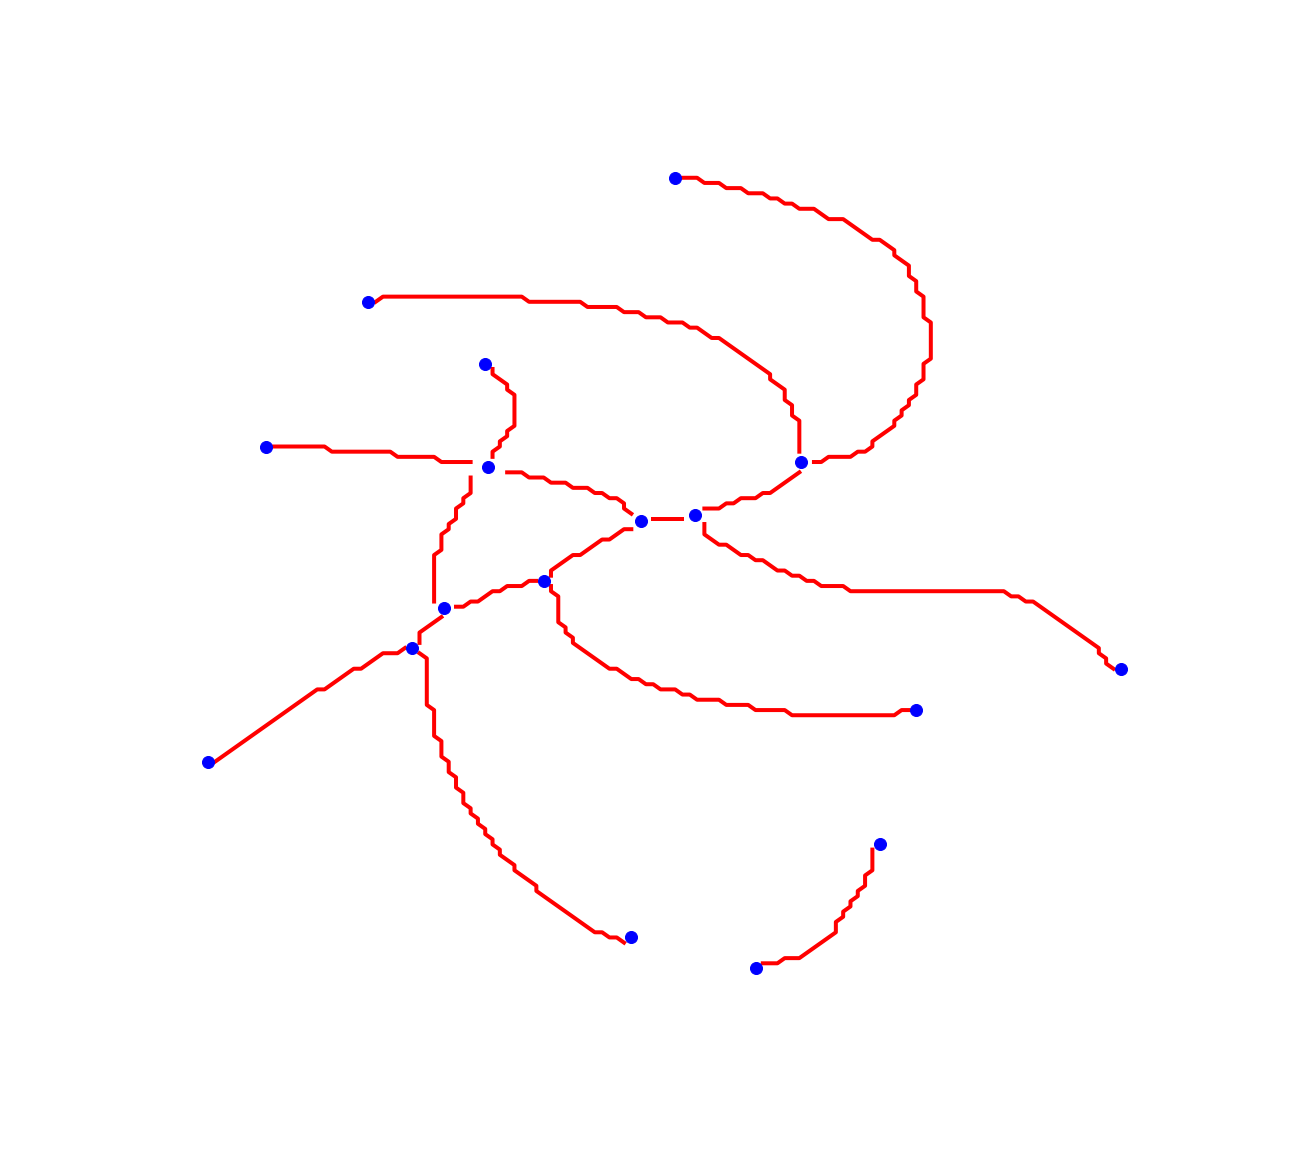
\includegraphics[height=1.5in]{graph_of_skel_no_axis.png}
        \caption{Grafo que representa la esqueletonizaci\'on de la red.}
        \label{Fig1d}
    \end{subfigure}
%    \vskip\baselineskip
    \caption{Procedimiento para obtener un grafo que representa la red, a partir del procesamiento de una imagen de microscop\'ia, utilizando segmentaci\'on y esqueletonizaci\'on. Fuente: \cite{breuer2015define}}
\end{figure*}
 
 
\section{Antecedentes}
\label{Antecedentes}
% Se sugiere agregar una sección para “Antecedentes” en donde se puedan describir conceptos relevantes en este trabajo. Por ejemplo, en la hipótesis se habla de múltiples métricas. Sin embargo no queda claro a qué se refiere ello. Estas definiciones podrían estar definidas dentro de “Antecedentes”
% En la sección de Antecedentes también se podrían describir los trabajos actuales relacionados con el problema.
% Indicar cuál es la intuición para relacionar un problema de Set Covering con extracción de filamentos. Sería bueno describir este punto en la propuesta. La definición de Set-Covering y su relación con este problema también podría estar en Antecedentes.

%Me fije que ahora explicas mas directamente set cover, pero la parte de la intuicion que relaciona con la imagen no es tan clara (en antecedentes y luego hipotesis).

Existen investigaciones en la literatura que apuntan a las distintas etapas de este problema, las que tienen en com\'un el uso de t\'ecnicas del \'area de procesamiento de im\'agenes para el tratamiento inicial de la imagen de microscop\'ia. La individualizaci\'on de filamentos puede ser categorizado en: basado en procesamiento de im\'agenes o como un problema de optimizaci\'on. 

\medskip
En la primera categor\'ia se encuentran enfoques asociados al an\'alisis de la reconstrucci\'on de filamentos en base a sus segmentos \cite{zhang2017extracting}, o relacionados a la extracci\'on de cada uno de los filamentos que conforman la red (\textit{Individual Fiber Segmentation}) a partir de una imagen \cite{doi:10.1021/ma502264c}\cite{boudaoud2014fibriltool}\cite{lichtenstein2003quantitative}\cite{alioscha2016robust}. Para estos m\'etodos, se han indicado como cr\'iticas la dificultad para identificar correctamente un filamento de otro, en los casos de  superposici\'on, fragmentaci\'on, o variaciones de intensidad en la imagen.
% describir alguno de estos papers 

En la segunda categor\'ia, \cite{cerda2014geometrical} plantea la identificaci\'on de segmentos de filamentos como un problema de asignaci\'on, utilizando las medidas de distancia euclidiana y angular como restricciones, y el algoritmo h\'ungaro para su resoluci\'on. En la misma categor\'ia, \cite{breuer2015define} realiza la asociaci\'on de la red con un grafo no dirigido con pesos, en el que cada filamento es equivalente a un camino en el grafo. Esto permite que la b\'usqueda e individualizaci\'on de filamentos, con un segmento de filamento representado por una arista del grafo, sumado a las restricciones que plantea el autor, sea tratado como un problema de {\it Set Cover}. En el caso de los m\'etodos de la segunda categor\'ia, la mayor cr\'itica es su costo computacional alto, lo que limita en parte aquel enfoque. Se debe agregar que los par\'ametros utilizados por estas t\'ecnicas (\'angulos o  distancias m\'aximas entre filamentos) son complejas de obtener de los expertos directamente. Sin embargo, una de sus ventajas es que automatizan la recuperaci\'on de informaci\'on incluyendo una mayor cantidad de propiedades a cada arista. 

%representa un camino en este grafo, y los conjuntos de caminos 
\medskip
%Todos estos enfoques, cuya entrada principal de datos son las im\'agenes etiquetadas a trav\'es de marcadores fluorescentes, 
% basados en grafos

A modo de ejemplo, el programa \texttt{DeFine} desarrollado en \cite{breuer2015define} describe el problema de identificaci\'on de filamentos como un problema de b\'usqueda de caminos, es decir, como un problema del tipo {\it Path Cover}. Se define el peso de cada segmento/arista por un c\'alculo de {\it aspereza}, asociada al ancho o intensidad de la arista o un conjunto de estas.
%, o tambi\'en puede ser calculado respecto al \'angulo entre aristas.
Este problema particular es llamado {\it Filament Covering Problem} (FCP) y los autores demuestran que es NP-Hard, por lo que proponen un algoritmo de aproximaci\'on mediante \textit{Set Cover}, cuyo objetivo es que cada arista pertenezca al menos a un conjunto. La definici\'on de {\it Set Cover} es:

\begin{quote}
Dado un conjunto de elementos, denominado universo, y $n$ conjuntos cuya unión comprende el universo, el {\it Set Cover Problem} consiste en identificar el menor n\'umero de conjuntos cuya unión a\'un contiene todos los elementos del universo.
\end{quote}

La adaptaci\'on a lo definido por {\it FCP} es: 
\begin{quote}
Sea el universo $U$ conformado por las aristas del grafo, y un conjunto $S$, conformado por conjuntos de aristas, cada uno con costo $c_s$, $s \in S$:

Encontrar un subconjunto $S_{set} \subseteq S$ con costo m\'inimo (o promedio, dependiendo de la forma en que se calcula la aspereza) tal que cada elemento en $U$ este cubierto al menos una vez.
\end{quote}

Con la demostraci\'on de que FCP es NP-Hard, dado que la cantidad de caminos crece de forma exponencial respecto al n\'umero de nodos, los autores de \cite{breuer2015define} plantean la elecci\'on de un subconjunto de caminos, con los que pueden expresar el problema de {\it Set Cover} como algoritmo de aproximaci\'on lineal fraccional binario. El subconjunto de caminos puede obtenerse con la heur\'istica de recorrer el grafo por su anchura ({\it Breadth-First Search}) deteniendose al momento que el \'angulo entre aristas supere 60$°$, o de caminos generados a partir de 100 \'arboles de expansi\'on m\'inima aleatoria ({\it RMST}), aportando cada uno de los 100 con $N(N-1)/2$ caminos no triviales y sin direcci\'on. 

Este enfoque faculta que al tener un grafo que representa la red de filamentos, como en la figura \ref{Fig1d}, sea posible llegar a resultados como los que aparecen en las figuras \ref{Fig2a} o \ref{Fig2b} a trav\'es de la asignaci\'on de pesos a la aristas, y de restricciones a las uniones entre diferentes las mismas. Cabe destacar que el {\it FCP} s\'olo utiliza 2 caracter\'isticas para describir los segmentos de los filamentos, siendo el \'angulo entre aristas usado en la etapa de selecci\'on de subconjuntos de caminos, y el ancho, empleado para describir el peso de las aristas.  
%es de complejidad $\mathcal{O}(N^{(2K+2)})$, con $N$ como n\'umero de nodos y $k$ como el n\'umero m\'aximo de caminos que pasan por cada v\'ertice. 
% Aquello permitir\'ia pasar de Fig1d a Fig2b por ejemplo

En ambas categor\'ias, las cr\'iticas m\'as repetidas en los trabajos del \'area suele ser la cantidad de par\'ametros y la dificultad en su ajuste, en las diversas herramientas existentes. Un segundo problema com\'un es que la obtenci\'on de informaci\'on relacionada a la morfolog\'ia y el comportamiento de las redes es m\'as cualitativo que cuantitativo \cite{asgharzadeh2018computational}\cite{qiu2014quantitative}, lo que supone un problema al trasladar el  an\'alisis a una gran cantidad de datos, dado que cada enfoque es demasiado espec\'ifico a su correspondiente software.

\medskip

\begin{figure*}[h]
    \begin{subfigure}[t]{0.5\textwidth}
        \centering
        
\includegraphics[height=1.2in]{define-weighted-4-expected2.png}
        \caption{Visualizaci\'on de un resultado posible de individualizaci\'on, limitando los filamentos identificados a estructuras simples.}
        \label{Fig2a}
    \end{subfigure}%
    ~ 
    \begin{subfigure}[t]{0.5\textwidth}
        \centering
        
\includegraphics[height=1.2in]{define-weighted-4-expected1.png}
        \caption{Visualizaci\'on de otro resultado posible de individualizaci\'on, permitiendo filamentos m\'as complejos.}
        \label{Fig2b}
    \end{subfigure}
	\caption{Posibles resultados de la identificaci\'on de filamentos. El resultado esperado de esta investigaci\'on es asociar a cada arista del grafo, como el de la figura \ref{Fig1d}, un peso que pondere diversos criterios como \'angulo de bifurcaci\'on del filamento, grosor, ancho y/o largo. Al plantearlo como un problema de optimizaci\'on, la ponderaci\'on y otras restricciones, entregar\'an resultados como la imagen \ref{Fig2a} o \ref{Fig2b}, expresado gr\'aficamente mediante gradiente de colores. Fuente: Elaboraci\'on propia}
\end{figure*}

%resolucion, cantidad parametros, descriptores, costo computacional
En resumen, el problema de identificar filamentos en im\'agenes de microscop\'ia esta limitado por la resoluci\'on, y los problemas de m\'ultiples par\'ametros a ajustar, para los m\'etodos basados en procesamiento de im\'agenes, el costo computacional en los m\'etodos basados en optimizaci\'on, y falta de descriptores cuantitativos en ambas. La revisi\'on bibliogr\'afica da cuenta tambi\'en de pocas herramientas disponibles. Todo lo anterior implica que parte del an\'alisis deba ser manual, lo que para grandes cantidades de datos, hace los estudios m\'as propensos a errores. 
%La falta de herramientas analíticas para cuantificar las estructuras sigue siendo un cuello de botella, ya que el análisis manual de grandes conjuntos de datos requiere una gran cantidad de tiempo y son propensos a sesgos y errores.
%Por otra parte, la soluci\'on a problemas de superposici\'on se soluciona mediante la sintonizaci\'on de par\'ametros, los que var\'ian dependiendo de la c\'elula observada. En el caso del uso de \textit{thinning} en una imagen, la informaci\'on respecto al grosor de la estructura se pierde.

\section{Preguntas de Investigaci\'on}

Como se ha presentado, los m\'etodos de individualizaci\'on de filamentos que s\'olo usan herramientas de procesamiento de im\'agenes, pueden representar la red a trav\'es de los filamentos que la conforman, sin embargo para el conteo de descriptores cuantitativos requieren de m\'ultiples par\'ametros. Por otra parte los m\'etodos de optimizaci\'on permiten reducir los par\'ametros, pero con un alto costo computacional, el que puede ser abordado con el uso de heur\'isticas o algoritmos de aproximaci\'on. 
En particular, el m\'etodo {\it FCP} presentado en la secci\'on \ref{Antecedentes}, utiliza s\'olo el ancho como caracter\'istica en la etapa de asignaci\'on de pesos a las aristas del grafo, lo que es usado en la funci\'on de minimizaci\'on del problema de optimizaci\'on planteado por ellos. En la etapa de selecci\'on del subconjunto de caminos, el mismo m\'etodo desarrolla una heur\'istica que utiliza {\it BFS} en conjunto con otra caracter\'istica, el \'angulo entre aristas.
Esto nos permite establecer la pregunta:
%El alumno de debe reordenar esta pregunta, partiendo por ejemplo de Recorrido de Grafos + Optimización sobre características de ancho, ángulo, etc como métodos para determinar la correcta cantidad de filamentos.
%2-4-26
\smallskip
¿Es posible determinar correctamente la cantidad de filamentos, desarrollando un modelo de optimizaci\'on que utilice una combinaci\'on de m\'ultiples caracter\'isticas como el largo, ancho, ángulo de bifurcación, curvatura o dirección, en la asignaci\'on de pesos como en la selecci\'on del subconjunto de caminos?
\smallskip

% costo computacional de m\'etodos de optimizaci\'on es abordado con algoritmos de aproximación o heurísticas
% Solucion actual propuesta en Define aborda el recorrido de grafos considerando como peso solo 1 valor que representa una caracteristica de la arista, 
% pregunta es si se puede determinar la cantidad de filamentos utilizando un peso que agrupe/pondere varias caracteristicas
%(geometricos comunmente)
% Entre las investigaciones y herramientas existentes derivadas de los mismos, 
%- overlap, intensidad, fragmentación

A aquella pregunta, se debe agregar que existe informaci\'on \textit{a priori}, indicada por el tipo de estructura observada, la cual restringe los comportamientos posibles de la red. Por ejemplo, los filamentos de prote\'ina actina no se pegan entre s\'i, formando estructuras sin ciclos, mientras que el ret\'iculo endoplasm\'atico (organelo celular encargado principalmente de la s\'intesis de prote\'inas) si presenta ciclos. Estas condiciones pueden aportar limites m\'as acotados a algunos de los criterios de cuantificaci\'on y es conocimiento disponible previo a la observaci\'on en el microscopio. Es importante destacar que alguna de la informaci\'on {\it a priori} corresponde a reglas emp\'iricas, que tambi\'en deben ser consideradas durante el an\'alisis.

%El ingreso de esta informaci\'on 
%- tampoco mencionas la dificultad de incorporar reglas empiricas de que es "a priori"
%acelerando el an\'alisis.
%length, orientation, position, width
% Metricas usadas solo algunos: Donde esta el paper? -> DeFine usa 1, MCerda usa 2 distancias, Asgardh2018 usa angulos, grossor, distancia 

\section{Hipótesis, Objetivos y Contribuci\'on}
\label{hipotesis}
Se plantea como hip\'otesis que a partir de un grafo que representa una red de filamentos, obtenido desde una imagen de microscop\'ia con t\'ecnicas descritas en la literatura, y utilizando una combinaci\'on de caracter\'isticas de los segmentos de filamentos como largo, ancho, \'angulo de bifurcaci\'on o curvatura, sumado a la incorporaci\'on de informaci\'on previa disponible sobre el tipo de c\'elula (red de filamentos con o sin ciclos), es posible identificar a cada filamento en la red resolviendo un modelo de optimizaci\'on.

Para validar esta hip\'otesis, se propone realizar los siguientes objetivos:
\subsection{Objetivo General}
Desarrollar un modelo de optimizaci\'on para la individualizaci\'on de filamentos a partir de un grafo representativo de la red de filamentos, evaluando la variaci\'on en el resultado 


con distintas ponderaciones entre las propiedades de cada segmento de filamento, como el ancho, largo, \'angulo de bifurcaci\'on y/o direcci\'on.
%y que incorpore la informaci\'on {\it a priori} disponible

\subsection{Objetivos Espec\'ificos}
\begin{itemize}
    \item Generar una formulaci\'on matem\'atica de un modelo de optimizaci\'on para la identificaci\'on de filamentos a partir de un grafo representativo de la red de filamentos. 
    \item Implementar un algoritmo que resuelva el modelo de optimizaci\'on, entregando como salida la identificaci\'on de filamentos, considerando casos de solapamiento y/o cruce.
    \item Identificar la ponderaci\'on de propiedades que entregue mejores resultados para grafos que representen una neurona, una bacteria y una c\'elula eucariota de planta. 
    
    %una soluci\'on exacta o aproximada respecto a la individualizaci\'on, dependiendo de la complejidad computacional del problema. 
\end{itemize}

\subsection{Contribuci\'on}

% Contribuci\'on:
Como resultado de los objetivos planteados, se obtendr\'a una herramienta para el an\'alisis automatizado de estructuras de filamentos, lo que permitir\'ia mejorar el seguimiento de procesos din\'amicos o la identificaci\'on de procesos patol\'ogicos de forma autom\'atica.
% pasar de Fig1d a Fig2a o Fig2b

\section{Metodolog\'ia}
%``I always thought something was fundamentally wrong with the universe'' \citep{adams1995hitchhiker}
% El segundo párrafo de la metodología no queda claro y es la que tiene relación con Set-Covering.
%* En una metodología es crítico especificar cómo se evaluará la propuesta (métricas) y este documento carece de ello. Se recomienda agregar esta información dentro de la metodología.

Para la realizaci\'on del estudio propuesto se realizar\'a una recopilaci\'on detallada del estado del arte relacionado a la identificaci\'on de filamentos, con enfoque en soluciones que utilicen no s\'olo herramientas de visi\'on por computador.
Por otra parte, el uso de software existente que provee pre-procesamiento de im\'agenes para la esqueletonizaci\'on y/o extracción de grafos que represente la estructura de la c\'elula, servir\'a de base para la obtenci\'on de ejemplos iniciales para realizar pruebas a la implementaci\'on del algoritmo. Estos programas presentan algunos de los problemas mencionados en las secciones anteriores, por lo que requerir\'an de adaptaciones para este trabajo.  

%A su vez, se incluir\'an en el estado del arte problemas basados en recorrer grafos para determinar el o los mejores caminos dado uno o m\'as criterios. 
%el {\it Path MTU Discovery} utilizado en redes para 

El n\'ucleo de la investigaci\'on estar\'a enfocado en desarrollar una formulaci\'on matem\'atica en la que las aristas del grafo contengan pesos asociados a la ponderaci\'on de m\'ultiples propiedades, como el largo, ancho, \'angulo de bifurcación y/o grosor, las que permitan identificar a los filamentos que componen la red a trav\'es del planteamiento de un modelo de optimizaci\'on, con el fin de clasificarlos correctamente con respecto a la subestructura a la que pertenecen, as\'i como determinar si el v\'ertice es parte de varias subestructuras simult\'aneamente o si se traslapa con otra.
La formulaci\'on deber\'a considerar balancear el peso de cada propiedad con respecto al peso final de cada arista, siendo este procedimiento lo m\'as autom\'atico posible, es decir, requiriendo la menor interacci\'on con el usuario. Otro aspecto a considerar ser\'a el costo computacional de la soluci\'on, que se ver\'a influido por el n\'umero de nodos en el grafo. En caso de que las los segmentos/aristas que constituyen el dominio de b\'usqueda para el modelo de optimizaci\'on sea demasiado grande, ser\'a necesario definir una heur\'istica que permita acotarlo.
% automatizacion de parametros?
%Es aqu\'i donde los problemas asociados de capacidad computacional pueden encontrarse

La construcci\'on del planteamiento matem\'atico considerar\'a tambi\'en ideas extra\'idas de problemas no directamente relacionados con la extracci\'on de filamentos, pero que se basan en grafos para calcular caminos \'optimos. Por ejemplo, problemas de redes de computadores para el c\'alculo de enrutamiento utilizan grafos con pesos. En particular, la forma en que se determina el peso de un {\it link} puede servir de base para desarrollar la ponderaci\'on de pesos buscada en este trabajo. A su vez, el uso de meta-heur\'isticas de inteligencia de enjambre como la colonia de hormigas puede servir para construir soluciones de forma din\'amica a medida que se evaluan diferentes aristas del grafo.
Con esta formulaci\'on se proceder\'a a construir un algoritmo que permita resolver el modelo de optimizaci\'on, obteniendo resultados cuantitativos en base a lo planteado en la hip\'otesis sobre un grafo que represente una estructura citoesqueletal. 

% COMO MEDIR LA CALIDAD
% Agregar test de hipotesis Kolgomorov Student t
Para la validaci\'on del algoritmo, se utilizar\'a como informaci\'on de entrada, im\'agenes sint\'eticas y luego im\'agenes reales. Adem\'as de realizar la extracci\'on del grafo que representa la red, las im\'agenes reales se encontrar\'an evaluadas por expertos, lo que establece el \textit{Gold Standard}, que es en este caso la identificaci\'on manual de filamentos realizada por el o los expertos contra la cual se realizar\'a la validaci\'on, dado que indica la cantidad correcta de filamentos, cruces y/o solapamientos.
Algunas de las im\'agenes reales provendr\'an de {\it papers} recopilados en la investigaci\'on del estado del arte, a modo de realizar una comparaci\'on con los resultados de los m\'etodos encontrados. Por su parte, las im\'agenes sint\'eticas permitir\'a medir la eficacia de la ponderaci\'on de propiedades respecto a casos iniciales de baja complejidad. Todo lo anterior permitir\'a establecer la cantidad de aciertos y errores del algoritmo.


%Dependiendo del avance del algoritmo, se llevara a cabo tambi\'en una comparaci\'on con m\'etodos similares existentes en la literatura. 
\bibliographystyle{plain}
\bibliography{references}

\end{document}
